\documentclass[../../main.tex]{subfiles}
\begin{document}
\noindent
\section{Cantilever Timoshenko beam with tip-body}

\textcolor{red}{MOONTLIK UIT HAAL.}

This section discusses a technical report [DBVXX]. In this technical report the authors models a cantilever Timoshenko beam with a tip body and elastic boundary conditions. This model can be seen as a motivation of the importance of investigating the validity of the Timoshenko beam theory.

This section discusses the model as presented in [DBVXX] as well as adding to the numerical results.

\subsection{The model problem}
Consider the dimensionless equations of motion \ref{eq:1D_Model:EquationOfMotion1D} and \ref{eq:1D_Model:EquationOfMotion2D} and constitutive equations \ref{eq:1D_Model:ConstitutiveEquations1D} and \ref{eq:1D_Model:ConstitutiveEquations2D} of a Timoshenko beam, as given in section \ref{sec:1D_Model}. The model in [DBVXX] adds two damping terms to these equations.


{Equations of Motion}
\begin{eqnarray}
	\partial_t^2 w &=& \partial_x V - c_1\partial_t w  + q, \label{CT_1}\\
	\frac{1}{\alpha}\partial_t^2 \phi &=& V+\partial_xM. \label{CT_2}
\end{eqnarray}

\noindent
{Constitutive Equations}
\begin{eqnarray}
	M &=& \frac{1}{\beta}\partial_x \phi +c_2 \partial_t \partial_x \phi,\label{CT_3}\\
	V&=& \partial_x w - \phi.\label{CT_4}
\end{eqnarray}

The term with $c_1$ models viscous damping and the term with $c_2$ models material damping.

\subsubsection{Boundary conditions}
It is assumed that the beam is elastically clamped at the endpoint $x=0$ and the tip-body is elastically clamped at the endpoint $x=1$.\\

The boundary conditions at the (elastically) clamped end $x=0$ are
\begin{eqnarray}
   w(0,t) &=&  0, \label{CT_5}\\
   M(0,t) &=&  \mu \phi(0,t). \label{CT_6}
\end{eqnarray}
The parameter $\mu > 0$ models the elastic interaction between the surface where the beam is attached and the beam itself. As $\mu$ increases, $\phi(0,t)$ decreases and similarly as $\mu$ decreases, $\phi(0,t)$ increases. Thus as $\mu$ increases, the join becomes ``more rigid" as the rotation of the cross-section is decreased. Obviously for a decrease in $mu$ the join becomes ``less rigid".\\

At the other endpoint where the tip body is attached, the following interface conditions derived by the authors of [DBVXX]
\begin{eqnarray}
- V(1,t) &=& m \partial_t^2 w(1,t) + md \ddot \theta(t) + k_1 \partial_t w(1,t) + k_1 d \dot \theta(t), \label{CT_7}\\
 -M(1,t) &=& J \ddot \theta(t) + d k_2 \dot \theta(t)- dV(1,t), \label{CT_8}\\
M(1,t) &=& \gamma (\theta(t)- \phi(1,t)). \label{CT_9}
\end{eqnarray}
In these equations, $m$ is the mass of the tip body, $J$ the moment of inertia about the centre of mass, $\theta$ represents the rotation of the tip- body, the terms with $k_1$ and $k_2$ are damping terms and $\gamma$ a parameter representing the elastic interaction between the tip body and the endpoint of the beam.\\

Similar to $\mu$, as $\gamma$ increases, $\theta(t) - \phi(1,t)$ decreases, hence the interaction is `more' rigid. And as $\gamma$ decreases, $\theta(t) - \phi(1,t)$ increases, so the interaction is `more' elastic. It is assumed that $\gamma > 0$.

\subsubsection{Remark}
The well-posedness of the model as well as the existence of unique solutions is investigated in [DBVXX].


\subsection{Variational form}
Let $f,g \in C[0,1]$. Multiplication and integration by parts results in
\begin{eqnarray}
\int_0^1~ \partial^2_t w(\cdot,t) f &=&  - \int_0^1~ V(\cdot,t)f' - c_1\int_0^1 \partial_t w(\cdot,t)f + \int_0^1q(\cdot,t)f \nonumber \\
& &+~V(1,t)f(1)~-~V(0,t)f(0), \label{CT_10}\\
 \int_0^1~ \frac{1}{\alpha}~\partial^2_t \phi(\cdot,t) g  &=& -\int_0^1~M(\cdot,t)g' + \int_0^1~ V(\cdot,t)g \nonumber\\
& & + M(1,t)g(1) -  M(0,t)g(0), \label{CT_11}
\end{eqnarray}

Let $h \in C[0,1]$. Multiply and integration gives:

\begin{eqnarray}
 \int_0^1 V(\cdot,t)h &=& \int_0^1 \partial_x wh - \int_0^1\phi h. \label{CT_12}
\end{eqnarray}

\subsubsection{Remark}
Integration by parts is not applied to equation \eqref{CT_12}. This results in the Mixed Finite Element Method.

Substituting the boundary conditions results in the following variational form
\begin{align}
\int_0^1~ \partial^2_t w(\cdot,t) f &=  - \int_0^1~ V(\cdot,t)f' - c_1\int_0^1 \partial_t w(\cdot,t)f + \int_0^1q(\cdot,t)f \nonumber \\
&  -(m \partial_t^2 w(1,t) +  md \ddot \theta(t) + k_1 \partial_t w(1,t)+ k_1 d \dot \theta(t))f(1) \nonumber\\
&~-~V(0,t)f(0), \label{CT_13}\\
 \int_0^1~ \frac{1}{\alpha}~\partial^2_t \phi(\cdot,t) g & = -\int_0^1\dfrac{1}{\beta} \partial_x \phi(\cdot,t)g' - c_2 \int_0^1 \partial_t \partial_x \phi(\cdot,t)g' +\int_0^1~V(\cdot,t)g \nonumber\\
 &  +\gamma \big(\theta(t) - \phi(1,t)\big)g(1) - \mu \phi(0,t)g(0), \label{CT_14}\\
 \int_0^1 V(\cdot,t)h &= \int_0^1 \partial_x wh - \int_0^1\phi h. \label{CT_15}
\end{align}

\subsubsection{Interface equation}
For the interface between the beam and tip body, the authors of [DBVXX] derive a differential equation for the interface at the tip body. Multiply the interface equation \eqref{CT_7} by d and add equation \eqref{CT_8} to obtain
\begin{align}
 J\ddot{\theta}(t) + dk_2\dot{\theta}(t) + dm\partial_t^2w(1,t) + md^2\ddot{\theta}(t) + dk_1\partial_tw(1,t) + k_1d^2\dot{\theta}(t)\nonumber \\
 = - \gamma(\theta(t)-\phi(1,t)) \label{CT_16}
\end{align}

\subsubsection*{Test functions}
The test function space can be defined as
\begin{align}
T[0,1] = \left\{ f \in C[0,1] ~~ | ~~ f(0)= 0~\right\} \label{CT_17}
\end{align}

Using the test function space and the variational form, it is possible to define a variational problem. Denote this problem by Problem Var.

\subsubsection{Problem Var} Find the functions $w$, $\phi$, $V$ and $\theta$ such that $\langle w(\cdot,t), \phi(\cdot,t) \rangle \in T[0,1] \times C^1[0,1]$, $V(\cdot,t) \in C^1[0,1]$ and $\theta(t) \in \mathbb{R}$ for all $t>0$ and the following equations hold:
\begin{align}
\int_0^1 \partial^2_t w(\cdot,t) f \ dx  & =   \int_0^1~ V(\cdot,t) f' \ dx - c_1\int_0^1 \partial_t w(\cdot,t)f \ dx + \int_0^1q(\cdot,t)f \ dx \nonumber \\
 &  -(m \partial_t^2 w(1,t) +  md \ddot \theta(t) + k_1 \partial_t w(1,t) + k_1 d \dot \theta(t))f(1), \label{CT_18}\\
\int_0^1 \frac{1}{\alpha}~\partial^2_t \phi(\cdot,t) g \ dx  &= -\int_0^1\dfrac{1}{\beta} \partial_x \phi(\cdot,t)g' \ dx - c_2 \int_0^1 \partial_t \partial_x \phi(\cdot,t)g' \ dx + \int_0^1 V(\cdot,t)g \ dx \nonumber \\
 &  +\gamma \big(\theta(t) - \phi(1,t)\big)g(1) - \mu \phi(0,t)g(0), \label{CT_19}\\
\int_0^1 V(\cdot,t)h \ dx &= \int_0^1 \partial_x w(\cdot,t)h \ dx - \int_0^1 \phi(\cdot,t)h \ dx,  \label{CT_20}
\end{align}
with the interface equation,
\begin{align}
(J+ md^2) \ddot \theta(t)+ (k_1d^2 + d k_2) \dot \theta(t)  + dm \partial_t^2 w(1,t)
  + dk_1 \partial_t w(1,t) \nonumber\\
  =  -\gamma \big(\theta(t) - \phi(1,t)\big),  \label{CT_21}
\end{align}

for all $f \in T[0,1]$ and $g,h \in C^1[0,1]$.\\




\subsection{Galerkin approximation}
Create a set of n+1 linear basis functions $\delta_i$, where $\delta_i \in C[0,1]$ for $i = 0,1,2,...,n$. Let $S_0 = \textrm{span}\left\{\delta_0,\delta_1,\delta_2,...,\delta_n\right\}$ and $S = \textrm{span}\left\{\delta_1,\delta_2,\delta_3,...,\delta_n\right\}$. 


\subsubsection{Problem G}
Find the functions $w^h$, $\phi^h$, $V^h$ and $\theta^h$ such that $w^h(\cdot,t) \in S$,  $\phi^h(\cdot,t),V^h(\cdot,t) \in S_0$ and $\theta^h(t) \in \mathbb{R}$ for all $t>0$ and the following equations hold:

\begin{align}
\int_0^1 \partial^2_t w^h(\cdot,t) \delta_i \ dx & =   \int_0^1 V^h(\cdot,t) \delta_i' \ dx - c_1 \int_0^1 \partial_t w^h(\cdot,t) \delta_i \ dx + \int_0^1 q(\cdot,t) \delta_i \ dx \nonumber \\
 & -(m \partial_t^2 w^h(1,t) +  md \ddot \theta^h(t)k_1 \partial_t w^h(1,t) + k_1 d \dot \theta^h(t))\delta_i(1), \\
\frac{1}{\alpha} \int_0^1 \partial^2_t \phi^h(\cdot,t) \delta_i \ dx & = -\dfrac{1}{\beta}\int_0^1\partial_x \phi^h(\cdot,t)\delta_i' \ dx - c_2 \int_0^1 \partial_t \partial_x \phi^h(\cdot,t) \delta_i' \ dx + \int_0^1 V^h(\cdot,t) \delta_i \ dx \nonumber \\
 & +\gamma \big(\theta^h(t) - \phi^h(1,t)\big)\delta_i(1) - \mu \phi^h(0,t)\delta_i(0),\\
\int_0^1 V^h(\cdot,t),\delta_i \ dx &= \int_0^1 \partial_x w^h(\cdot,t) \delta_i \ dx -  \int_0^1 \phi^h(\cdot,t) \delta_i \ dx, 
\end{align}
for $i = 0,1,2,...,n+1$.\\

And the interface equation,
\begin{align}
(J+ md^2) \ddot \theta^h(t)+ (k_1 d^2 + d k_2) \dot \theta^h(t)  + dm \partial_t^2 w^h(1,t)
  + dk_1 \partial_t w^h(1,t) \nonumber\\
  =  -\gamma \big(\theta^h(t) - \phi^h(1,t)\big).
\end{align}

\subsection{System of ordinary differential equations}
Consider the following standard Finite Element matrices
\begin{align*}\label{ch6_eq10}
M_{ij} = \int_0^1 \delta_j \delta_i, ~K_{ij} = \int_0^1 \delta'_j\delta'_i ~\textrm{and} ~L_{ij} = \int_0^1 \delta_j\delta'_i.
\end{align*}

Using the matrices $M$, $K$ and $L$, Problem G can be rewritten as a system of ordinary differential equations. This system is referred to as Problem ODE.

\subsubsection{Problem ODE}
Find the functions $\bar{w} \in S$, $\bar{\phi}, \bar{V} \in S_0$ and $\theta^h \in \mathbb{R}$ such that
\begin{align}
M_w\ddot{\bar{w}} = L_w\bar{V} -\big(m \ddot{w}_{n+1}(t) + k_1 \dot{w}_{n+1}(t) \big)\delta_i(1) + M^* \bar{q}(t) + \bar{q}_I,\\
\label{sys2}
\frac{1}{\alpha} M \ddot{\bar{\phi}} = -\frac{1}{\beta} K\bar{\phi} + M\bar{V} + \tilde{G},\\
\label{sys2.1}
\bar{0} = -M\bar{V} + L^T\bar{w} - M\bar{V}.
\end{align}

With the interface equation
\begin{align} \label{sys3} \nonumber
(J+md^2) \ddot \theta^h(t) &+ (d k_2+ d^2 k_1 ) \dot \theta^h(t)  + dm {\ddot w}_{n+1}(t) +  dk_1 {\dot w}_{n+1}(t)\\
  =&  -\gamma \big(\theta^h(t) - {\phi}_{n+1}(t)\big).
\end{align} and $\bar{q}_I$ the interpolation of the function $q$ over the basis functions.


\subsection{Numerical results}
These equations can be rewritten in a general form for a system of ordinary differential equations
\begin{align}
	A\ddot{\bar{u}} &= B\dot{\bar{u}} + C\bar{u} + D
\end{align}
and
\begin{align}
	a \ddot{\theta} & = b \dot{\theta} + c \theta + d
\end{align} with $\bar{u} = \langle \bar{w}, \bar{\phi}, \bar{V} \rangle$.\\

A finite difference scheme can be applied to find $\bar{u}$ and $\theta$ numerically. An example of a scheme that can be used is the Central Difference Average Acceleration finite difference method. The following results were obtained by implementing a MATLAB program.\\

The beam is excited using a periodic forcing function $q(t) = 0.1 \sin(\frac{\pi}{4}t)$ to induce motion. The damping parameters are set to $c_1 = 0$, $c_2 = 0$, $k_1 = 0.1$ and $k_2 = 1$.

\newpage
\FloatBarrier
\subsubsection{Case: Control}
Consider the control case as presented in [DBVXX].\\

 The maximum displacement is $u$ is 0.07694. And the maximum angle of cross-section at tip-body is 0.005552.

\begin{figure}[!hb]
\makebox[\textwidth]{
\centering
 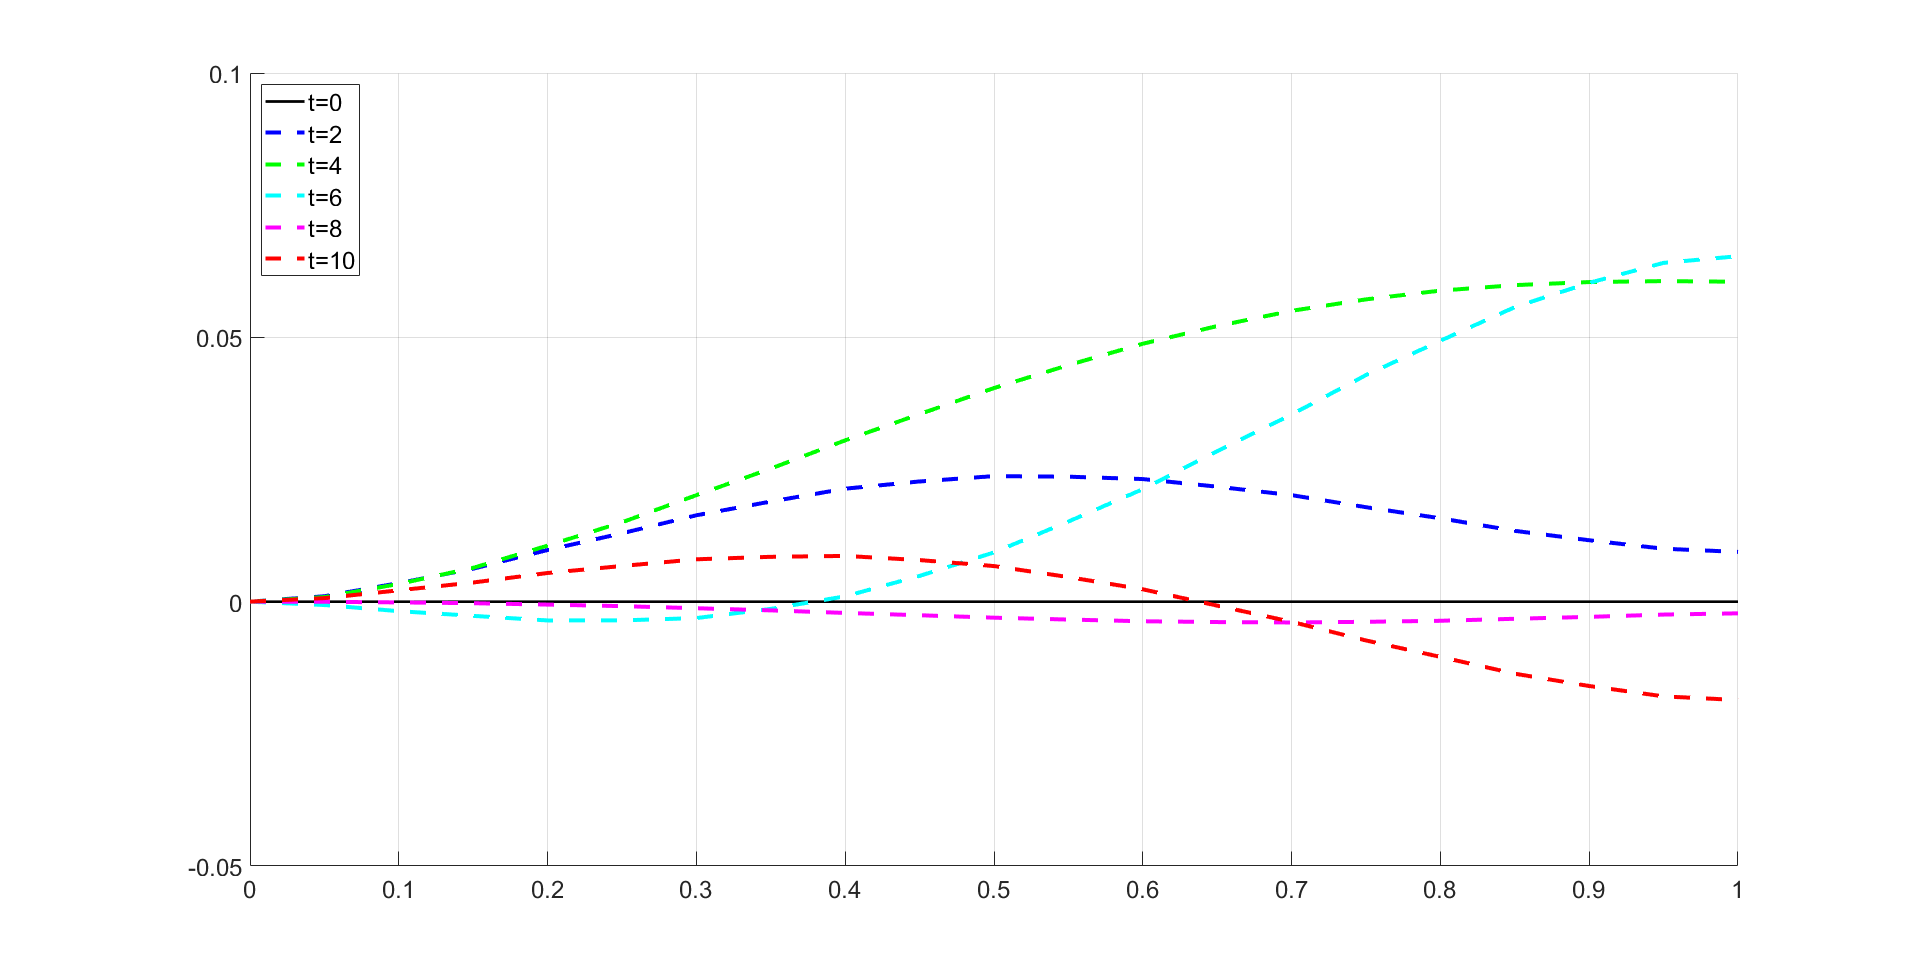
\includegraphics[scale=0.3]{../../images/TimoshenkoTipBody/ControlMotion.png}
 \caption{Motion of the beam with $\mu = 0.5$, $\gamma = 0.5$, $m = 0.1$}\label{CLB_F5}}
\end{figure}

\begin{table}[!hb]
\makebox[\textwidth]{
\renewcommand{\arraystretch}{1}
    \begin{tabular}{|c||c||c||c||}
        \hline
         t & $\phi(1)$ & $\theta$ & $\phi(1) - \theta$\\ 
        \hline
        0  & 0 & 0 & 0 \\
        2  & -0.002020353467526 & -0.000027406615955 & -0.001992946851571 \\
        4  & -0.000596779278874 & -0.000134256143882 & -0.000462523134992 \\
        6  & 0.004742324601643 	& -0.000810001256052 & 0.005552325857694 \\
        8  & 0.000059161424311 	& -0.001289328238416 & 0.001348489662727 \\
        10 & -0.003024749574431 & -0.000359603287124 & -0.002665146287307 \\
        \hline 
        \end{tabular}
        \caption{Angle of the beam and tip-body at time $t$ and their relative error.}\label{CLB_T1}}
\end{table}

\FloatBarrier
\subsubsection{Case: Decrease $\gamma$}
For this case, the parameter $\gamma$ is decreased. Compared to the control case, the maximum angle achieved of the cross-section at the tip body is increased.\\

The maximum displacement is $u$ is 0.07801. And the maximum angle of cross-section at tip-body is 0.02676.

\begin{figure}[!hb]
	\makebox[\textwidth]{
		\centering
		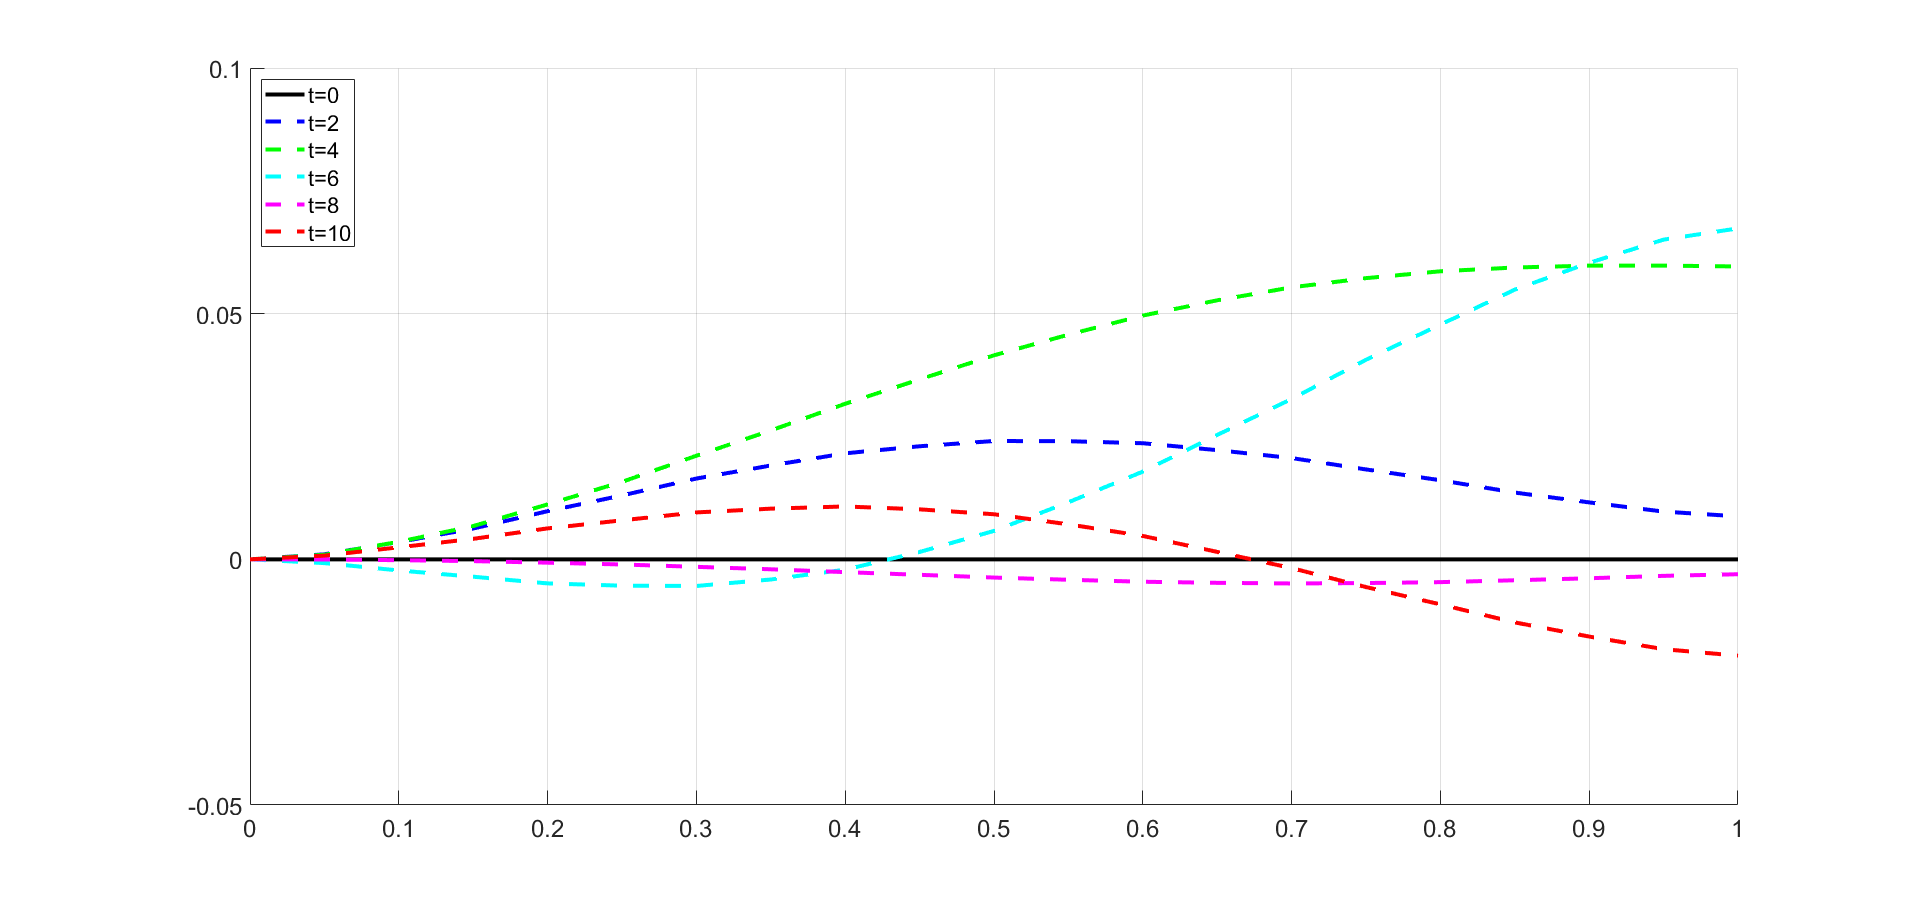
\includegraphics[scale=0.3]{../../images/TimoshenkoTipBody/ControlMotion_gam.png}
		\caption{Motion of the beam with $\mu = 0.5$, $\gamma = 0.1$, $m = 0.1$}\label{CLB_F5}}
\end{figure}

\begin{table}[!hb]
	\makebox[\textwidth]{
		\renewcommand{\arraystretch}{1}
		\begin{tabular}{|c||c||c||c||}
			\hline
			t & $\phi(1)$ & $\theta$ & $\phi(1) - \theta$\\ 
			\hline
			0  & 0 & 0 & 0 \\
			2  & -0.008968780504176 & -0.000034622649348 & -0.008934157854828 \\
			4  & -0.003421432704948 & -0.000247657709436 & -0.003173774995512 \\
			6  & 0.025401485816257 	& -0.001090880083035 & 0.026492365899293 \\
			8  & 0.004576031105634 	& -0.002083479267232 & 0.006659510372866 \\
			10 & -0.015386157002644 & -0.002074203805624 & -0.013311953197020 \\
			\hline 
		\end{tabular}
		\caption{Angle of the beam and tip-body at time $t$ and their relative error.}\label{CLB_T1}}
\end{table}

\FloatBarrier
\subsubsection{Case: Decrease $\mu$}
For this case, the parameter $\mu$ is decreased. Compared to the control case, the maximum displacement of the beam achieved during motion is increased..\\

The maximum displacement is $u$ is 0.08017. And the maximum angle of cross-section at tip-body is 0.005854.

\begin{figure}[!hb]
	\makebox[\textwidth]{
		\centering
		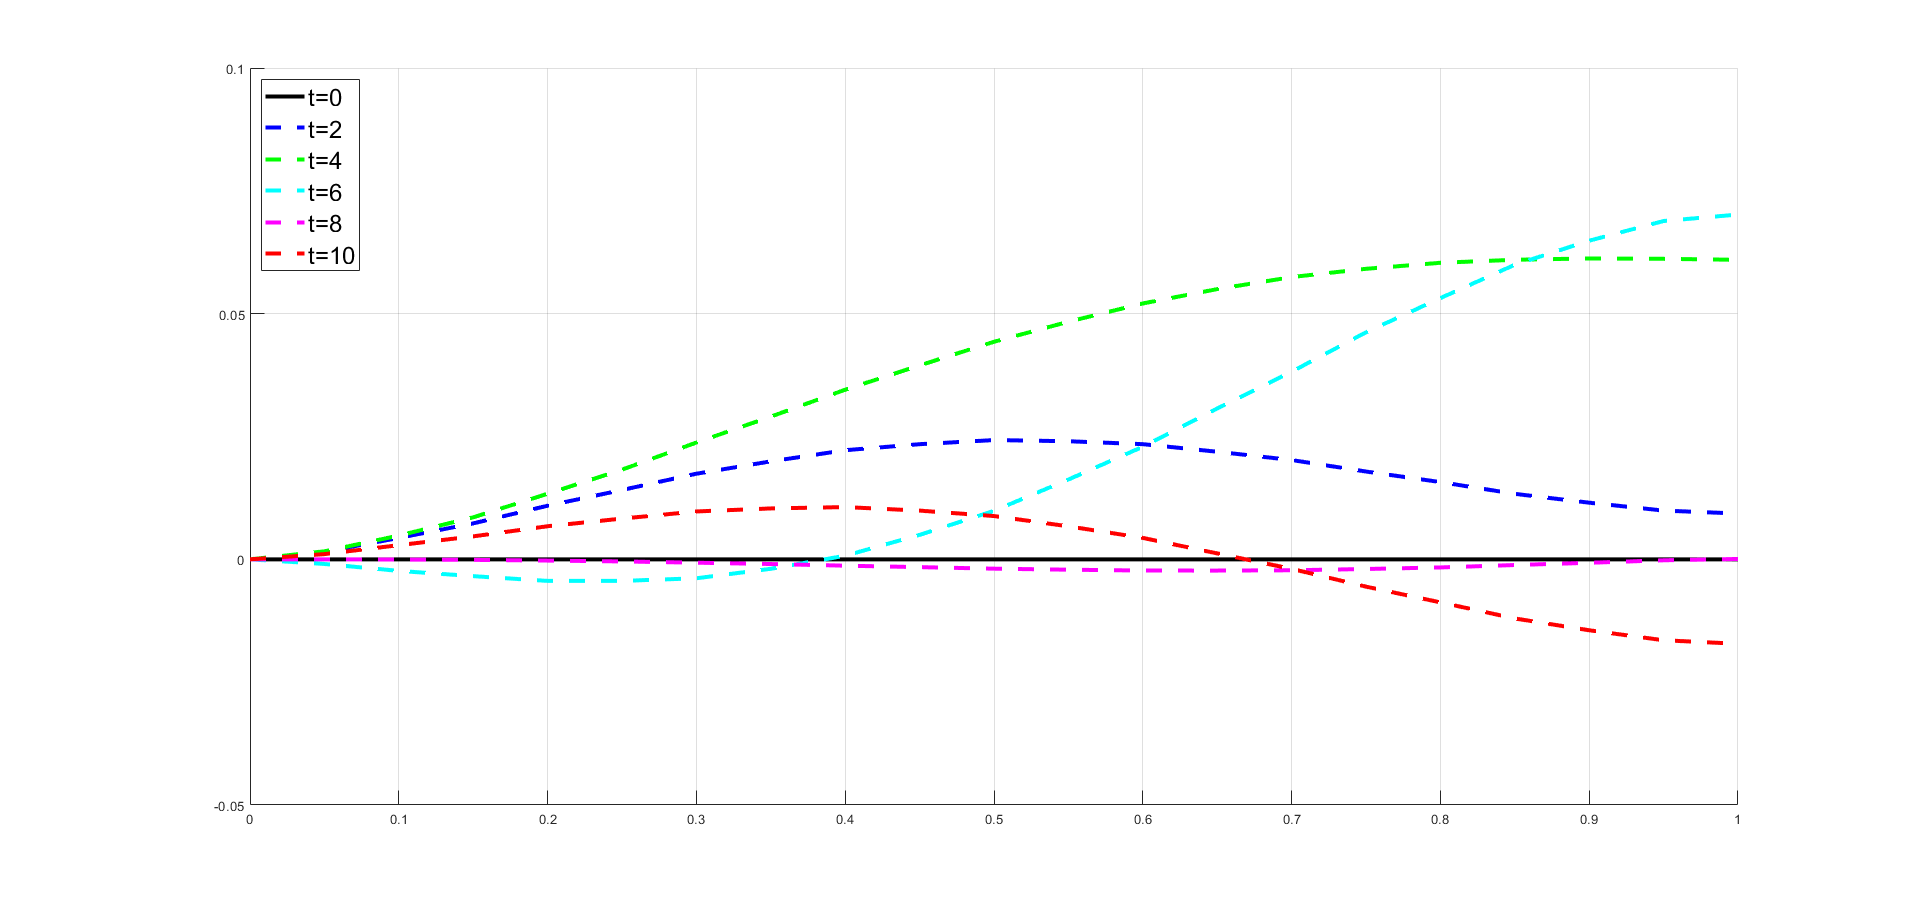
\includegraphics[scale=0.3]{../../images/TimoshenkoTipBody/ControlMotion_mu.png}
		\caption{Motion of the beam with $\mu = 0.1$, $\gamma = 0.5$, $m = 0.1$}\label{CLB_F5}}
\end{figure}

\begin{table}[!hb]
	\makebox[\textwidth]{
		\renewcommand{\arraystretch}{1}
		\begin{tabular}{|c||c||c||c||}
			\hline
			t & $\phi(1)$ & $\theta$ & $\phi(1) - \theta$\\ 
			\hline
			0  & 0 & 0 & 0 \\
			2  & -0.0020146527231596 & -0.000026854667752 & -0.001987798055407 \\
			4  & -0.000919770985602 & -0.000102876004834 & -0.000816894980768 \\
			6  & 0.005023665668264 	& -0.000752726666843 & 0.005776392335107 \\
			8  & 0.000210040029687 	& -0.001352805739549 & 0.001562845769236 \\
			10 & -0.003254467815569 & -0.000453217154384 & -0.002801250661185 \\
			\hline 
		\end{tabular}
		\caption{Angle of the beam and tip-body at time $t$ and their relative error.}\label{CLB_T1}}
\end{table}

\FloatBarrier
\subsubsection{Case: Increase $m$}
For this case, the parameter $m$ is increased. This parameter represents the weight of the tip body. Compared to the control case, the maximum displacement of the beam achieved during motion is decreased. Lag in the motion of the beam can also be seen in Figure \ref{lag}. \\

The maximum displacement is $u$ is 0.04813. And the maximum angle of cross-section at tip-body is 0.007164.

\begin{figure}[!hb]
	\makebox[\textwidth]{
		\centering
		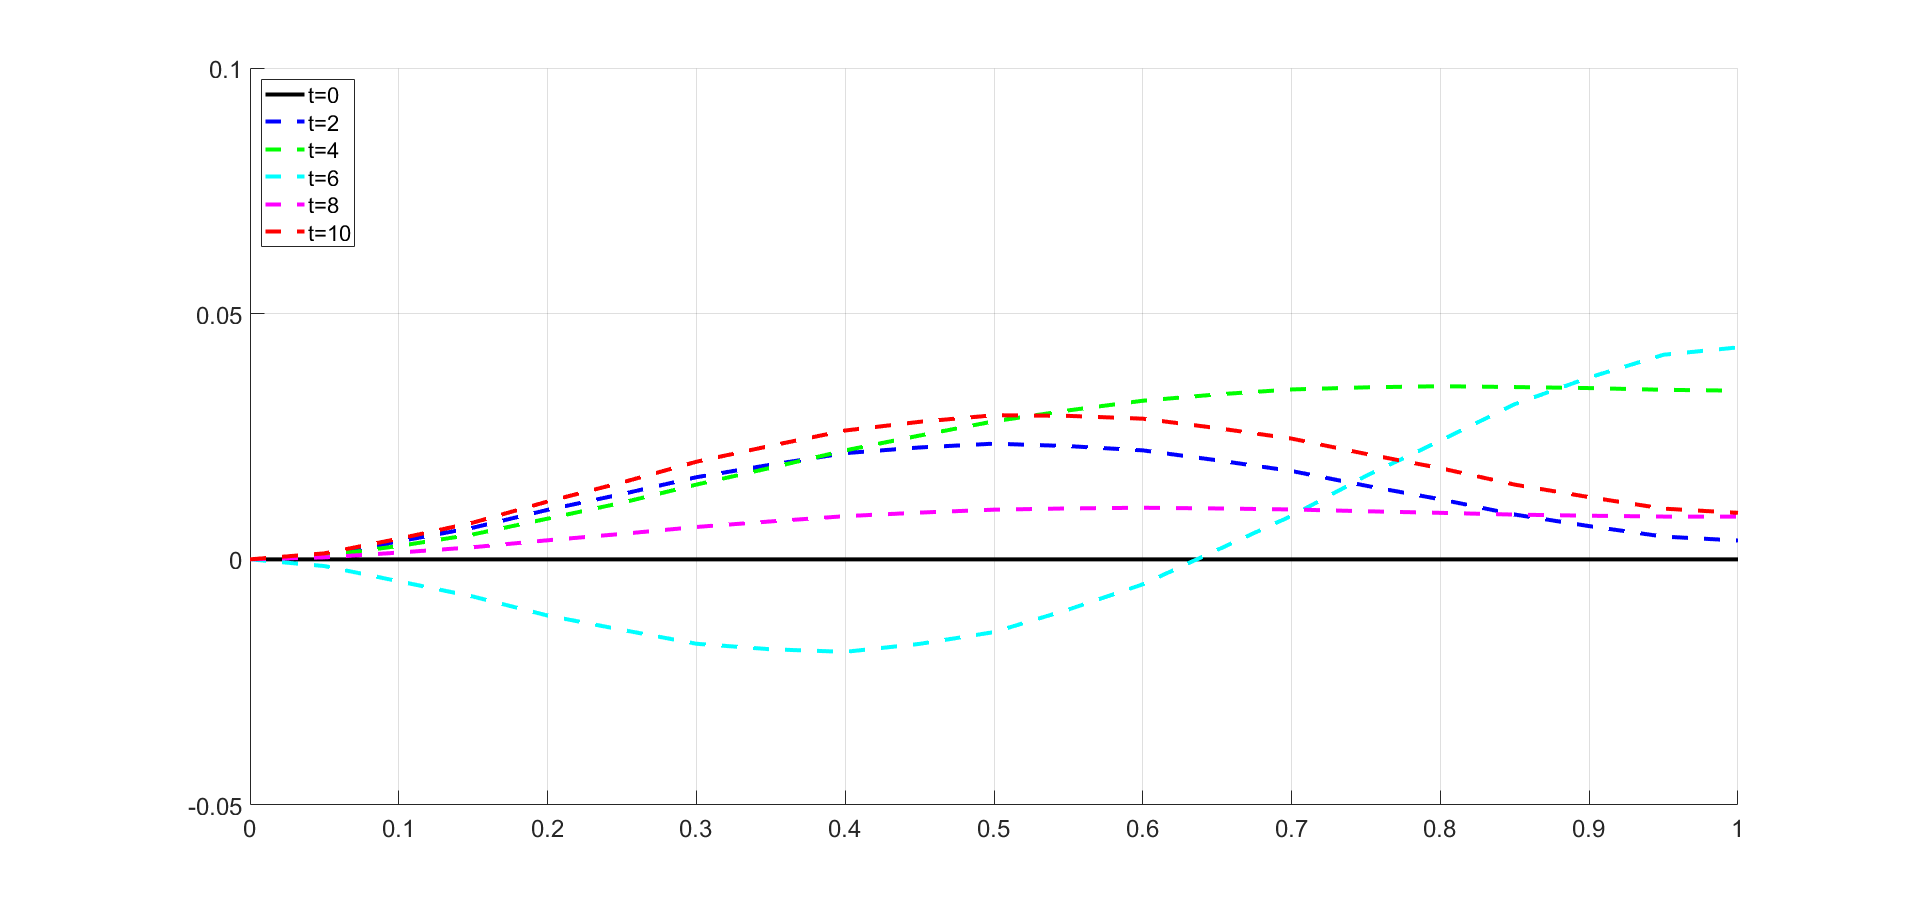
\includegraphics[scale=0.3]{../../images/TimoshenkoTipBody/ControlMotion_m.png}
		\caption{Motion of the beam with $\mu = 0.5$, $\gamma = 0.5$, $m = 0.5$}\label{lag}}
\end{figure}


\begin{table}[!hb]
	\makebox[\textwidth]{
		\renewcommand{\arraystretch}{1}
		\begin{tabular}{|c||c||c||c||}
			\hline
			t & $\phi(1)$ & $\theta$ & $\phi(1) - \theta$\\ 
			\hline
			0  & 0 & 0 & 0 \\
			2  & -0.001872928034631 & 0.000860073660995 & -0.002733001695626 \\
			4  & 0.000838496309022 & 0.002376699454088 & -0.001538203145066 \\
			6  & 0.000527590593005 	& -0.006558345806040 & 0.007085936399045 \\
			8  & -0.000248514461727 	& -0.0009904383205016 & 0.000741923858774 \\
			10 & -0.000030840351397 & 0.003708628513388 & -0.003739468864785 \\
			\hline 
		\end{tabular}
		\caption{Angle of the beam and tip-body at time $t$ and their relative error.}\label{CLB_T1}}
\end{table}

\end{document}
